\documentclass[a4paper,titlepage]{article}
\usepackage[utf8]{inputenc}
\usepackage[T1]{fontenc}
\usepackage[portuguese,provide=*]{babel}
\usepackage{url}
\usepackage{graphicx}
\usepackage{microtype}
\usepackage[labelfont=bf]{caption}
\usepackage[labelfont=bf]{subfig}
\usepackage{amsmath, amssymb, geometry, setspace, float}
\usepackage{mathtools,empheq}
\usepackage[pagebackref=true,breaklinks=true,letterpaper=true,colorlinks,bookmarks=false]{hyperref}

\newlength{\topToTitle}
\setlength{\topToTitle}{30pt}
\newlength{\leftToTitle}
\setlength{\leftToTitle}{-50pt}
\newlength{\titleToInfo}
\setlength{\titleToInfo}{6cm}
\newlength{\myTextWidth}
\setlength{\myTextWidth}{\textwidth}
\advance\myTextWidth by 1.5cm

\newenvironment{changemargin}[2]{%
  \begin{list}{}{%
    \setlength{\topsep}{0pt}%
    \setlength{\leftmargin}{#1}%
    \setlength{\rightmargin}{#2}%
    \setlength{\listparindent}{\parindent}%
    \setlength{\itemindent}{\parindent}%
    \setlength{\parsep}{0pt plus 1pt}%
  }\item}{\end{list}}

\begin{document}\hypersetup{pageanchor=false}\begin{titlepage}
\enlargethispage{100pt}
\begin{changemargin}{-0.5cm}{-1cm}
\renewcommand{\title}{%
  {\LARGE Utilização de Dados de Vídeo}\\
  {\LARGE Aplicados à Visão Computacional}\\[4pt]
  \mbox{Visualizando Informações de Vídeo no Formato AV1}
}
\renewcommand{\author}{Prof.\ Ricardo Fabbri, Ph.D.}
\renewcommand{\date}{\today}
\newcommand{\info}{%
  \raisebox{4pt}[-4pt]{%
  
\includegraphics[height=1.3cm]{figs/logo-iprj2.eps}
  \hspace{0.1in}
  }\\

  Grupo de Visualização\\
  Instituto Politécnico -- IPRJ\\
  Universidade do Estado do Rio de Janeiro\\[1.5cm]

  Nova Friburgo, \date\\[1.5cm]

  \textbf{Orientador}\\[4pt]
  Prof.\ Ricardo Fabbri, Ph.D.\\[8pt]
  \textbf{Aluno}\\[4pt]
  Bernardo Brust Toledo Pereira\\[8pt]
  \textbf{Projetos Relacionados}\\[4pt]
   FAPERJ Jovem Cientista do Nosso Estado E25/2014 204167\\
   FAPERJ APQ1 01/09335-8\\
   FAPERJ E28/2014/204747\\
   UERJ Prociência 2014--2017
}

\vspace*{\topToTitle}
\begin{minipage}{\myTextWidth}
  \sffamily
  \hspace*{\leftToTitle}\begin{minipage}{11cm}
    \Large\textbf{Projeto de Iniciação Científica}\\[1.5cm]
    \title\\[1.5cm]
    \author
  \end{minipage}\\

  \vspace*{\titleToInfo}

  \begin{minipage}{\textwidth}
    \flushright
    \info
  \end{minipage}
\end{minipage}
\end{changemargin}
\end{titlepage}
\hypersetup{pageanchor=true}
\onehalfspacing

\providecommand{\keywords}[1]
{
  \small
  \textbf{\textit{Palavras-chave---}} #1
}

\providecommand{\areaname}[1]
{
  \small
  \textbf{\textit{Nome da área, subárea e especialidade---}} #1
}

\areaname{Computação}

\keywords{Processamento de Vídeo, Visão Computacional, Software Livre}

\section{Introdução e Justificativa}

O presente plano de pesquisa refere-se a atividades propostas para a Iniciação Científica (IC), a serem realizadas no Laboratório de Visualização do Instituto Politécnico (IPRJ) da UERJ, vinculado ao Departamento de Modelagem Computacional (DMC). O objetivo central é expandir o escopo de pesquisa do laboratório, integrando o processamento e a análise de vídeo ao arsenal de ferramentas que atualmente foca primordialmente em imagens estáticas. Tal avanço será suportado pela construção de ferramentas de fácil integração para análise de vídeos, servindo como ponto de entrada para futuras investigações sobre os benefícios deste formato de mídia.

O vídeo consolidou-se como uma das formas predominantes de comunicação digital. Com o avanço de plataformas de \emph{streaming}, a popularização das redes sociais e a maturidade da indústria de jogos, os casos de uso de conteúdo audiovisual são onipresentes. Nesse contexto, é fundamental que a visão computacional desfrute dos benefícios que esse formato oferece em relação ao uso de imagens estáticas.

Fundamentalmente, vídeos são sequências de imagens apresentadas em rápida sucessão~\cite{videodismistified}. Assim, técnicas consolidadas, como a reconstrução 3D a partir de imagens, podem ser adaptadas para vídeos, desde que as adequações necessárias sejam executadas. No entanto, é possível ir além: formatos modernos de compressão, como o AV1, utilizam técnicas avançadas de redução de redundância, como a \emph{inter prediction}. Esta técnica representa partes do quadro por deslocamentos em relação a regiões de referência, em vez de repetir todos os seus pixels~\cite{aomedia2021av1}. Os vetores de movimento associados a esses blocos, embora otimizados para predição e não para medir fluxo óptico, são uma fonte potencialmente valiosa de pistas temporais para aplicações de visão computacional~\cite{computer_vision,av1motion}.

Para explorar esse potencial, são necessárias ferramentas eficientes e robustas que permitam a visualização de vetores de movimento, canais de cores e relações temporais entre quadros (\emph{frames}). Tais ferramentas são úteis não apenas para análise direta, mas também para a integração em projetos futuros que explorem a visão computacional em vídeo~\cite{av1motion}.

Os \emph{codecs} são softwares responsáveis por encodificar e decodificar formatos específicos de vídeo. Por exemplo, o \emph{codec} de formato AV1 pode tanto produzir vídeos AV1 a partir de dados visuais (encodificação), como gerar os dados visuais a partir do arquivo de vídeo (decodificação). A figura~\ref{fig:Diagrama_encodificacao} demonstra o processo de encodificação para o codec AV1 e similares:

\begin{figure} [H]
	\centering
	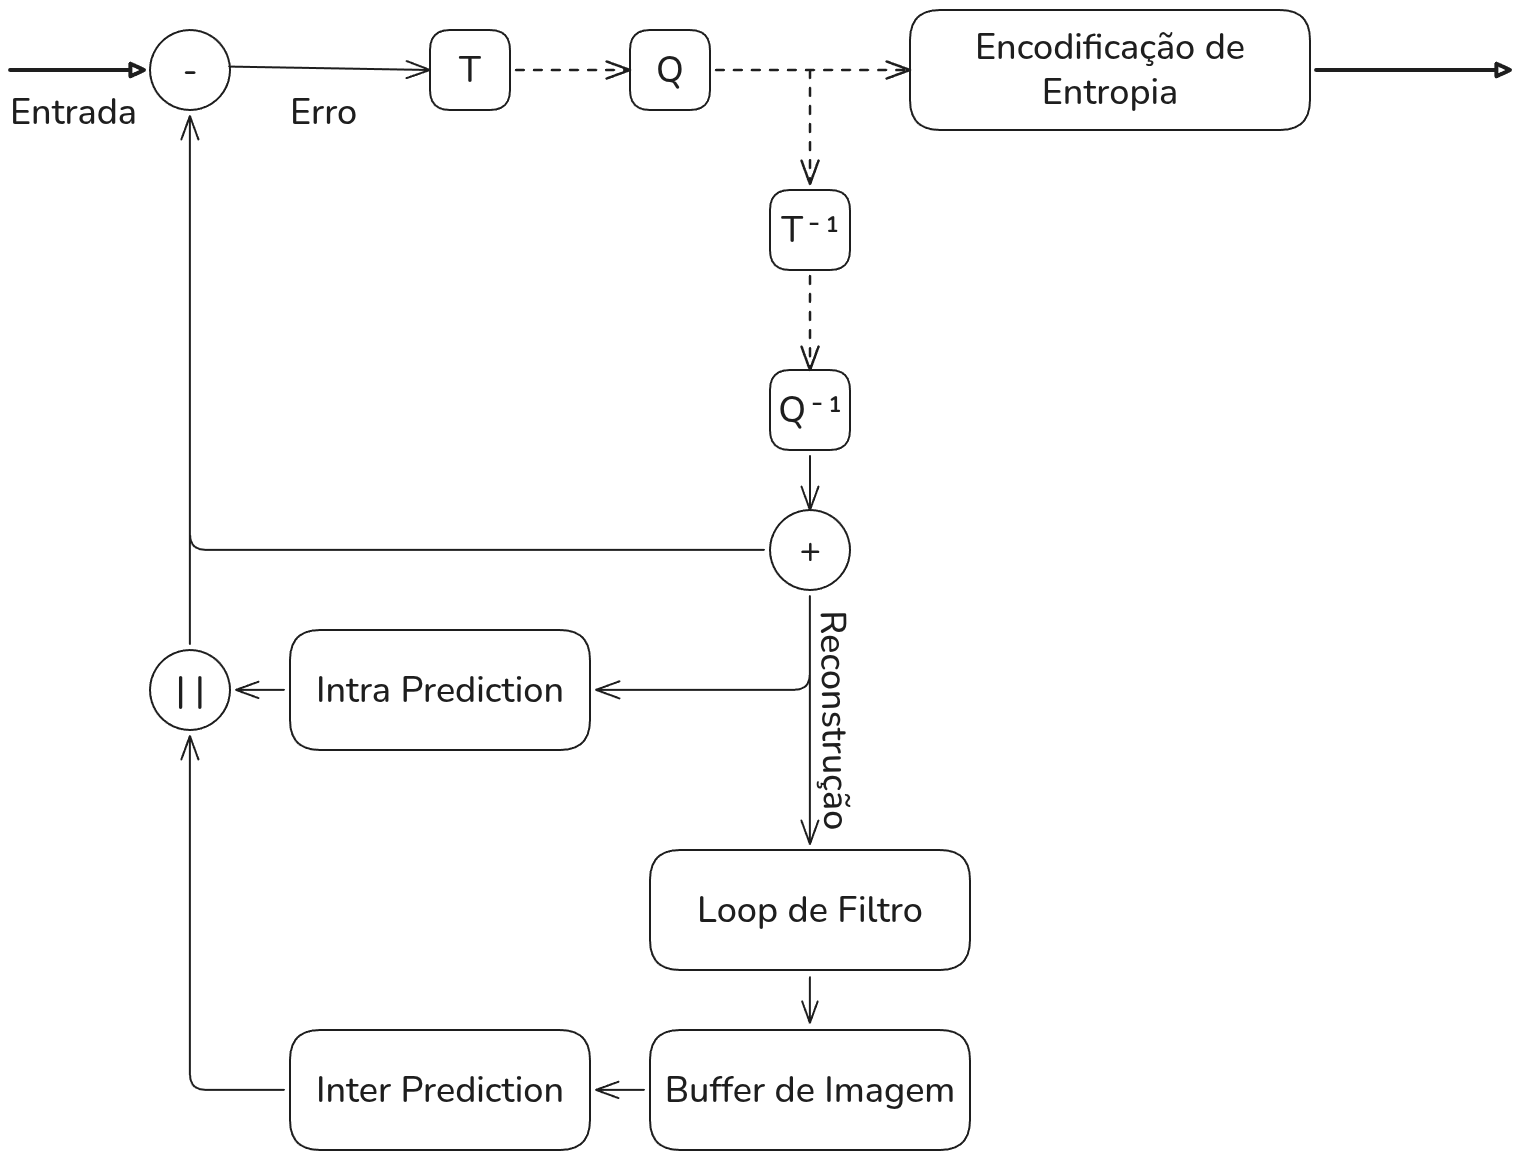
\includegraphics[width=1\linewidth]{figs/Diagrama_encodificacao.png}
	\caption{
    Diagrama demonstrando o processo de encodificação de vídeo.
	}\label{fig:Diagrama_encodificacao}
\end{figure}

As etapas funcionam da seguinte maneira:
\begin{itemize}
    \item \textbf{Entrada}: O ponto de entrada da encodificação é onde o \emph{codec} recebe os dados visuais puros que serão comprimidos. No ciclo do diagrama, estamos considerando um quadro (imagem) por vez como entrada.
    \item \textbf{T}: Depois de escolher uma predição intra ou inter, o codificador transforma o sinal residual (a diferença entre o bloco original e a predição). No AV1 podem ser usadas transformadas separáveis, como DCT, ADST, FLIPADST e identidade, em tamanhos que variam com a partição do bloco. A transformada concentra a energia do residual em poucos coeficientes, mas, por si só, é reversível.
    \item \textbf{Q}: A quantização reduz a precisão dos coeficientes transformados, usualmente por divisão e arredondamento controlados pelo parâmetro de quantização. Esta é uma das principais fontes de perda: coeficientes de alta frequência pouco perceptíveis podem tornar-se zero. A escolha adaptativa de tamanho de transformada, predição e quantização determina a relação taxa--distorção do quadro.
    \item \textbf{T inversa e Q inversa}: O codificador reconstrói localmente o quadro a partir dos coeficientes quantizados para manter um estado idêntico ao que o decodificador terá. A desquantização e a transformada inversa não recuperam exatamente o original, pois a quantização é irreversível; por isso a predição de quadros seguintes usa referências reconstruídas, e não a imagem de entrada.
    \item \textbf{Loop de Filtro}: Na reconstrução, o AV1 aplica filtros no laço de referência, incluindo \emph{deblocking}, \emph{CDEF} (\emph{constrained directional enhancement filter}) e \emph{loop restoration}. Eles reduzem artefatos de blocos e \emph{ringing} antes de o quadro entrar no conjunto de referências, melhorando tanto a qualidade visual quanto a eficiência das predições posteriores.
    \item \textbf{Buffer de Imagem}: Esta etapa armazena imagens anteriormente encodificadas para serem utilizadas posteriormente em \emph{Inter Prediction}.
    \item \textbf{\emph{Inter Prediction}}: Esta é uma das etapas mais relevantes para o projeto. O AV1 particiona o quadro em \emph{superblocks} de até $128\times128$ amostras, subdivididos recursivamente em blocos. Para cada bloco inter, o codificador pode escolher uma ou duas imagens de referência, estimar um vetor de movimento com precisão fracionária, e compensar o movimento por interpolação. Também são possíveis predição composta, movimento global e transformações afins locais (\emph{warped motion}). O vetor e o residual codificado descrevem como reconstruir o bloco; eles não constituem, portanto, uma medida direta e necessariamente densa do movimento físico da cena.
    \item \textbf{\emph{Intra Prediction}}: Em blocos intra, a predição usa amostras já reconstruídas nas bordas superior e esquerda do mesmo quadro. O AV1 dispõe de modos direcionais, \emph{smooth}, \emph{Paeth}, \emph{palette} e \emph{chroma from luma} (CfL), entre outros. Esses modos exploram estrutura espacial e correlação entre luma e croma sem depender de outro quadro.
    \item \textbf{Codificação de Entropia}: Os símbolos sintáticos --- modos de predição, vetores, coeficientes e índices --- são comprimidos por codificação aritmética baseada em distribuições cumulativas adaptativas. Esta etapa é sem perdas: a perda de informação decorre sobretudo da quantização e de decisões de modelagem anteriores, não da codificação entrópica.
\end{itemize}

\subsection{Aspectos técnicos do AV1 relevantes ao projeto}

AV1 é um padrão de bitstream desenvolvido pela Alliance for Open Media. Um arquivo pode ser encapsulado, por exemplo, em WebM ou ISO BMFF, enquanto o fluxo comprimido é formado por \emph{Open Bitstream Units} (OBUs). Entre elas estão unidades de cabeçalho de sequência, cabeçalhos e dados de quadro, metadados e delimitadores temporais. O cabeçalho de sequência informa propriedades globais, como perfil, dimensões máximas, profundidade de bits, subamostragem de croma e ferramentas habilitadas; os cabeçalhos de quadro descrevem, entre outros campos, o tipo de quadro, referências e parâmetros de quantização~\cite{aomedia2021av1}.

Os quadros podem ser \emph{key frames}, \emph{inter frames}, \emph{intra-only frames} ou \emph{switch frames}. Um \emph{key frame} pode iniciar uma nova cadeia de referência; quadros inter exploram referências passadas e, conforme a ordem de apresentação e decodificação, também referências futuras. O padrão mantém até sete referências nomeadas e separa a ordem de apresentação da ordem de decodificação. Essa distinção é indispensável ao visualizador: um quadro pode ser decodificado antes de ser apresentado e, portanto, a aplicação deve usar marcas de tempo, e não a ordem de chegada dos pacotes, para exibi-lo corretamente.

Para o escopo de visão computacional, três limitações devem ser consideradas. Primeiro, os vetores são definidos por blocos de tamanhos variáveis e podem apontar para referências que não são o quadro imediatamente anterior; a sobreposição deve registrar bloco de origem, bloco de destino, referência e escala temporal. Segundo, áreas ocluídas, regiões sem textura e decisões de taxa-distorção podem produzir vetores descontínuos ou escolhidos para economizar bits, e não para representar o deslocamento real. Terceiro, predição composta e movimento global podem fazer com que um bloco possua mais de uma hipótese de movimento. Consequentemente, a avaliação proposta comparará os vetores extraídos com métodos de \emph{optical flow} e \emph{SfM}, em vez de assumi-los como verdade de referência~\cite{av1motion}.

\section{Principais Objetivos}

Este projeto visa proporcionar ao aluno experiência com técnicas modernas de processamento de vídeo digital, decodificação de alta performance utilizando ferramentas como o \emph{FFmpeg}~\cite{ffmpeg}, e análise de dados em visão computacional. O foco central será o desenvolvimento de ferramentas de extração e visualização de dados de vídeos no formato AV1.

O formato AV1 é de particular interesse para este projeto: ele é um formato aberto e isento de royalties. Isso significa que o \emph{codec} do formato tem seu código fonte disponível na internet de forma gratuita para uso e estudo. Ademais, estudos realizados pela Meta apontam que o formato é superior aos seus concorrentes em usos práticos~\cite{metastudy}.

Em relação ao hardware a ser utilizado, a decodificação AV1 é computacionalmente exigente, podendo ser realizada na CPU, de forma relativamente lenta, porém viável com ferramentas como \emph{FFmpeg}~\cite{ffmpeg}, ou por aceleração de hardware quando disponível. Para os propósitos deste trabalho, em que a decodificação em tempo real não é requisito, a ferramenta será programada para suportar a decodificação em CPU, solução mais acessível e reprodutível.

O sistema processará vídeos em formato AV1 para produzir representações gráficas dos dados presentes nos vídeos, como os vetores de movimento gerados durante a codificação, além de informações como canais de cores e sombreamento~\cite{aomedia2021av1}.

Os objetivos específicos incluem:
\begin{itemize}
    \item Avaliar a precisão dos vetores de movimento gerados pelo \emph{codec} para fins de visão computacional.
    \item Investigar a utilidade desses vetores em tarefas como a reconstrução 3D (\emph{SfM}: \emph{Structure from Motion}).
    \item Comparação com outras técnicas de \emph{SfM} denso e \emph{optical flow}~\cite{av1motion}.
    \item Analisar a viabilidade de determinar vetores de movimento em cenários com grandes deslocamentos nas posições da câmera.
    \item Explorar o uso de canais de croma para compreender a geometria de objetos com poucos detalhes.
    \item Avaliar a viabilidade de adaptar os métodos já utilizados no laboratório para o vídeo~\cite{trifocal_problem}.
    \item Desenvolver uma ferramenta de código aberto que possibilite a visualização desses dados e sua integração em sistemas de pesquisa existentes.
\end{itemize}

\begin{figure} [H]
	\centering
	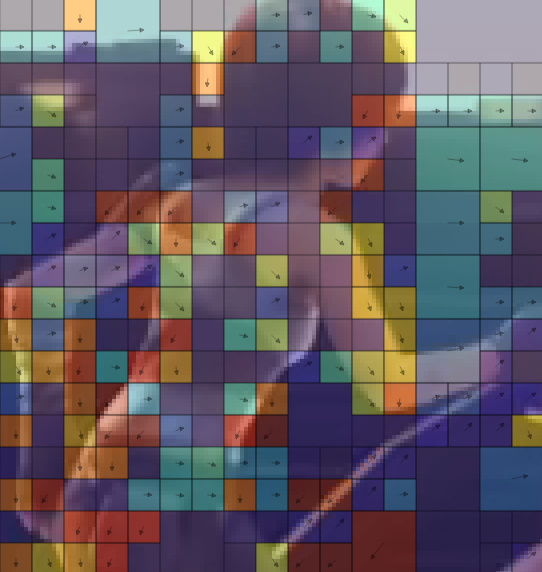
\includegraphics[width=1\linewidth]{figs/statistics_crop.png}
	\\ \small{Fonte: ``Video Coding Basics - How is this so efficient? - Por Christian Feldmann''}
	\caption{
    Exemplo de visualização da \emph{Intra Prediction} realizada no canal de luma de um vídeo encodificado em H.265. Vale notar que o formato AV1 realiza previsões melhores que as do H.265~\cite{metastudy}.
	}\label{fig:statistics_crop}
\end{figure}

A figura~\ref{fig:statistics_crop} apresenta um possível produto da ferramenta. Os vetores apresentados indicam uma diferença no comportamento da luz entre o quadro anterior e o atual. Tal campo vetorial é de suma importância para visualização aplicada à reconstrução 3D.

\section{Principais Atividades e Metodologia}

A execução do projeto será dividida nas seguintes etapas:

\begin{itemize}
    \item \textbf{Construção da Camada de Plataforma:} Desenvolvimento da base do visualizador, incluindo a camada de plataforma, interface de usuário e interação.
    \item \textbf{Implementação do Visualizador de Vídeo:} Desenvolvimento das funcionalidades de inspeção, como reprodução quadro a quadro, câmera lenta e visualização lado a lado, utilizando a biblioteca \emph{FFmpeg}~\cite{ffmpeg} para decodificação na CPU.
    \item \textbf{Extração e Overlay de Dados:} Implementação da renderização de vetores de movimento e outros metadados diretamente sobre o vídeo.
    \item \textbf{Visualização de Canais Adicionais:} Inclusão de funcionalidades para visualizar canais de cores, croma e outros dados estruturais.
    \item \textbf{Investigação dos Efeitos em Bordas e Regiões com Baixa Textura:} Estudo do comportamento dos canais auxiliares em objetos de baixo detalhe. Como o uso de sombreamento para percepção de profundidade.
    \item \textbf{Otimização e Validação:} Análise de desempenho via \emph{profiling} e garantia de qualidade por meio de testes automatizados.
    \item \textbf{Documentação e Publicação:} Disponibilização do código-fonte em repositório público, acompanhado de estudos de caso e guias de integração.
\end{itemize}

As etapas serão conduzidas de forma incremental. Inicialmente, será construída uma versão mínima capaz de abrir um arquivo AV1, decodificar seus quadros e apresentá-los na ordem temporal correta. Sobre essa base, serão incorporados os mecanismos de inspeção e as camadas de dados auxiliares. A cada incremento, serão utilizados vídeos curtos e controlados para verificar a coerência entre os dados extraídos, a imagem apresentada e a interação oferecida pela ferramenta. Essa estratégia permite isolar problemas de decodificação, sincronização e visualização antes da realização dos experimentos de análise de movimento.

\subsection{Integração com a API do FFmpeg}

A integração será feita diretamente com as bibliotecas \texttt{libavformat}, \texttt{libavcodec} e \texttt{libavutil}, em vez de invocar o executável \texttt{ffmpeg} como processo externo. Essa decisão permite que o visualizador controle o fluxo de pacotes e quadros na memória, preserve metadados por quadro e se integre à interface gráfica sem arquivos intermediários. A \texttt{libavformat} identifica o contêiner e realiza o \emph{demuxing}; a \texttt{libavcodec} seleciona e executa o decodificador AV1; e a \texttt{libavutil} fornece estruturas, opções e rotinas auxiliares compartilhadas~\cite{ffmpeg}.

O caminho básico de decodificação será: (i) abrir a entrada com \texttt{avformat\_open\_input} e obter as informações dos fluxos; (ii) localizar o fluxo de vídeo AV1 e copiar seus parâmetros para um \texttt{AVCodecContext}; (iii) abrir o decodificador disponível; (iv) ler \texttt{AVPacket}s com \texttt{av\_read\_frame}; (v) enviar cada pacote ao decodificador por \texttt{avcodec\_send\_packet}; e (vi) receber todos os \texttt{AVFrame}s disponíveis com \texttt{avcodec\_receive\_frame}. O protocolo de envio e recebimento é essencial porque um pacote pode gerar nenhum, um ou vários quadros, e porque há atraso interno causado por reordenação e por dependências entre referências. Ao final da leitura, o envio de um pacote nulo drena os quadros ainda retidos no decodificador.

Cada \texttt{AVFrame} será tratado como uma imagem planar YUV, e não como um vetor RGB contíguo. Os ponteiros \texttt{data[]} e os passos \texttt{linesize[]} descrevem os planos de luma e croma, que podem ter profundidade de 8, 10 ou 12 bits e subamostragem como 4:2:0. Essa representação será preservada na análise para evitar conversões desnecessárias e para permitir a inspeção separada dos canais. Quando a interface gráfica exigir RGB, a conversão será explicitamente feita com \texttt{libswscale}, respeitando a matriz de cores, a faixa de valores e as características de croma sinalizadas pelo fluxo.

A sincronização será baseada no \texttt{PTS} do quadro, convertido da \emph{time base} do fluxo para uma unidade comum. Essa escolha permite reprodução correta em taxas de quadro variáveis e em vídeos com ordem de decodificação distinta da ordem de apresentação. A ferramenta também manterá o índice sequencial de decodificação, pois ele é útil para depuração, mas não o confundirá com o tempo de apresentação.

Para a extração de movimento, a implementação verificará os \emph{side data} associados ao \texttt{AVFrame}, em particular \texttt{AV\_FRAME\_DATA\_MOTION\_VECTORS}. Os registros de movimento serão convertidos para uma estrutura própria que armazene posição e dimensões do bloco, deslocamento, referência e \texttt{PTS}. Os outros dados relacionados a compressão podem ser extraídos de forma similar.

\subsection{Protocolo de avaliação}

Os experimentos utilizarão vídeos AV1 com diferentes resoluções, taxas de quadro, níveis de quantização e padrões de movimento. Serão incluídas sequências com deslocamentos predominantemente translacionais, movimentos de câmera, oclusões, bordas bem definidas e regiões de baixa textura. Para cada vídeo, serão preservados os parâmetros de codificação, a ordem de apresentação dos quadros e as referências empregadas, de modo que os resultados possam ser reproduzidos e interpretados em função das decisões do \emph{codec}.

Os vetores extraídos serão visualizados sobre os quadros de origem e comparados, quando aplicável, com estimativas produzidas por métodos de \emph{optical flow} e \emph{SfM}. A comparação considerará a direção e a magnitude dos deslocamentos, a continuidade espacial do campo vetorial, a cobertura dos blocos e o comportamento nas regiões em que a predição temporal é menos confiável. Como os vetores de movimento do AV1 são produzidos para fins de compressão, a avaliação será qualitativa e quantitativa, buscando identificar condições em que eles constituem uma aproximação útil para tarefas de visão computacional, e não uma medida exata do movimento físico~\cite{av1motion,computer_vision}.

Também serão avaliados o tempo de abertura do arquivo, a taxa de decodificação, o consumo de memória e a responsividade das operações de inspeção. Os testes de desempenho serão executados com configurações de entrada registradas, permitindo distinguir limitações da implementação de limitações inerentes à resolução, à profundidade de bits ou à estrutura de predição do vídeo.

\subsection{Validação e resultados esperados}

A validação funcional verificará se a ferramenta apresenta os quadros segundo seus \texttt{PTS}, permite navegação quadro a quadro e mantém a correspondência entre cada sobreposição e o quadro ao qual ela pertence. Serão incluídos testes automatizados para rotinas de leitura de metadados, conversão de coordenadas, tratamento de referências e ordenação temporal. Casos sem vetores disponíveis ou com formatos de croma distintos deverão ser tratados explicitamente, sem comprometer a reprodução do vídeo.

Como resultado, espera-se obter um visualizador reutilizável para inspeção de vídeos AV1 e um conjunto documentado de procedimentos para extrair e analisar seus dados auxiliares. Os resultados experimentais indicarão tanto as situações em que os vetores de movimento podem apoiar aplicações de reconstrução e análise geométrica quanto suas limitações em cenas com oclusões, baixa textura ou movimentos complexos. O código, os vídeos de teste permitidos para distribuição e a documentação de uso serão organizados para facilitar sua integração em investigações futuras do laboratório.

\section{Cronograma}

O cronograma de atividades está dividido em quatro etapas semestrais:

\begin{center}
\begin{tabular}{|l|c|c|c|c|}
\hline
\textbf{Atividades / Semestres} & \textbf{1} & \textbf{2} & \textbf{3} & \textbf{4} \\ \hline
Construção da Camada de Plataforma & X & & & \\ \hline
Implementação do Visualizador de Vídeo & X & X & & \\ \hline
Extração e Overlay de Dados & & X & X & \\ \hline
Investigação dos Efeitos em Bordas e Regiões com Baixa Textura & &   & X & X \\ \hline
Otimização e Validação & & & X & X \\ \hline
Documentação e Publicação & & X & X & X \\ \hline
\end{tabular}
\end{center}

\section{Conclusão}

Este projeto propõe a exploração de técnicas modernas de visualização de dados aplicadas à análise de vídeo. Além de capacitar o aluno no estado da arte da visão computacional, o trabalho atende a uma demanda por ferramentas que auxiliem na transição do processamento de imagens estáticas para o vídeo. O formato AV1, sendo aberto e de rápida adoção, representa um cenário ideal para esta investigação. Espera-se que a ferramenta desenvolvida contribua significativamente para a área, possibilitando aplicações futuras em reconstrução 3D em tempo real e análise geométrica baseada em dados de compressão.

\vspace{1cm}

\bibliographystyle{ieeetr}
\bibliography{personal}

\end{document}
